\section{Generic ARQ implementation}\label{sc:overall}

The ARQ stop-and-wait method has been implemented on all nodes in the system. Figure \ref{fig:tohopornotarqsequence} is a sequence diagram of the  protocol implementation and shows how data requests are initiated by the base station and forwarded either directly to the runner  (left side) or via a relay station (right side).

\begin{figure}[H]
	\centering
	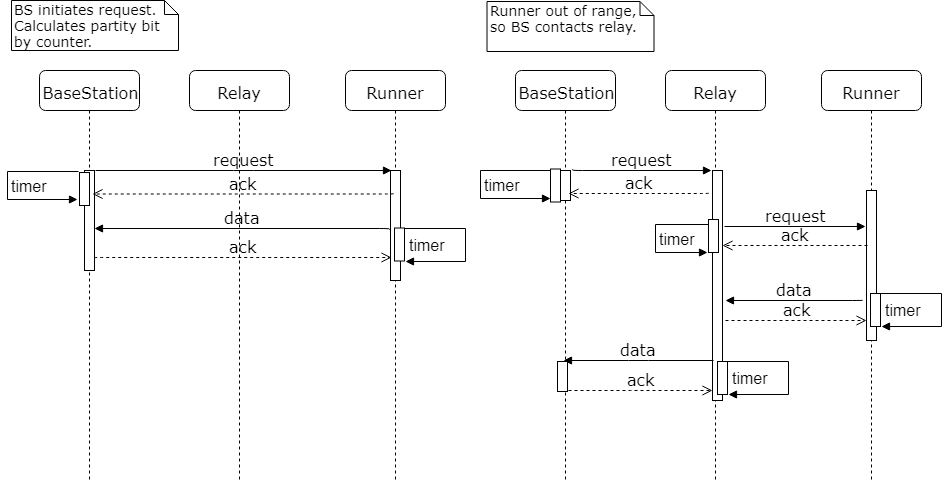
\includegraphics[width=1\linewidth]{implementation/overall/toHopOrNotArqSequence}
	\caption{The flow of data and acknowledgment messages between the nodes.}
	\label{fig:tohopornotarqsequence}
\end{figure}

